\documentclass[11pt]{article}
\def\activityid{FACILITATOR v2}% Week 1 v2. Shared style and exact unit-edge geometry.
\usepackage[letterpaper,margin=.65in,top=.60in,bottom=.65in]{geometry}
\usepackage[T1]{fontenc}
\usepackage[default]{sourcesanspro}
\usepackage{microtype,tikz,array,tabularx,fancyhdr,amsmath}
\usepackage[hidelinks]{hyperref}
\usetikzlibrary{calc,arrows.meta}
\setlength{\parindent}{0pt}\setlength{\parskip}{7pt}
\setlength{\headheight}{0pt}\setlength{\footskip}{26pt}
\setlength{\emergencystretch}{2em}
\pagestyle{fancy}\fancyhf{}\renewcommand{\headrulewidth}{0pt}\renewcommand{\footrulewidth}{.4pt}
\fancyfoot[L]{\scriptsize Bellingham Math Circle / Week 1 / \activityid}
\fancyfoot[R]{\scriptsize \thepage}
\definecolor{ink}{gray}{.12}\definecolor{soft}{gray}{.95}\color{ink}
\newlength{\blockside}\setlength{\blockside}{1in}
\def\hh{0.8660254037844386}
\tikzset{outline/.style={draw=ink,line width=1.05pt,line join=round},tile/.style={draw=ink,line width=.65pt,line join=round},gridline/.style={draw=black!40,line width=.35pt}}
\newcommand{\HexPath}{(-1,0)--(-.5,-\hh)--(.5,-\hh)--(1,0)--(.5,\hh)--(-.5,\hh)--cycle}
\newcommand{\BluePath}{(0,0)--(1,0)--(1.5,\hh)--(.5,\hh)--cycle}
\newcommand{\ChevronPath}{(0,0)--(1,0)--(1.5,\hh)--(1,2*\hh)--(0,2*\hh)--(.5,\hh)--cycle}
\newcommand{\BoardPath}{(0,0)--(1,0)--(2,2*\hh)--(1,4*\hh)--(0,4*\hh)--(-1,2*\hh)--cycle}
\newcommand{\PageTitle}[2]{{\fontsize{10}{12}\selectfont\bfseries WEEK 1\quad TILING LAB\hfill #1\par}\vspace{3pt}{\fontsize{27}{30}\selectfont\bfseries #2\par}\vspace{2pt}}
\newcommand{\NameLine}{{\small Name: \rule{2.65in}{.4pt}\hfill Date: \rule{1.35in}{.4pt}\par}\vspace{4pt}}
\newcommand{\Task}[2]{\par\vspace{3pt}{\large\bfseries #1}\par #2\par}
\newcommand{\Subhead}[1]{\par\vspace{3pt}{\large\bfseries #1}\par}
\newcommand{\RuleBox}[1]{\par\begingroup\setlength{\fboxsep}{8pt}\colorbox{soft}{\parbox{\dimexpr\linewidth-16pt\relax}{#1}}\endgroup\par}
\newcommand{\WriteBox}[2]{\par\textbf{#1}\par\vspace{2pt}\begin{tikzpicture}\draw[black!40,line width=.5pt] (0,0) rectangle (\dimexpr\linewidth-.5pt\relax,#2);\end{tikzpicture}\par}
\newcommand{\DrawOutline}[1]{\begin{tikzpicture}[x=\blockside,y=\blockside]\draw[outline] #1;\end{tikzpicture}}
\newcommand{\Pair}[1]{\par\vspace{4pt}\begin{minipage}[t]{.485\linewidth}\centering\textbf{First filling}\par\vspace{8pt}\DrawOutline{#1}\end{minipage}\hfill\begin{minipage}[t]{.485\linewidth}\centering\textbf{Another filling}\par\vspace{8pt}\DrawOutline{#1}\end{minipage}\par}
\newcommand{\ScaleCheck}{\vfill\par\begingroup\fontsize{9}{11}\selectfont\begin{minipage}[c]{1.2in}\centering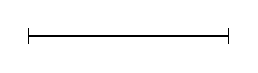
\begin{tikzpicture}[x=\blockside,y=1in]\draw[line width=.65pt] (0,0)--(1,0);\draw (0,-.04)--(0,.04) (1,-.04)--(1,.04);\end{tikzpicture}\par One small block edge\end{minipage}\hfill\begin{minipage}[c]{\dimexpr\linewidth-1.35in\relax}Adult: print \textbf{100\% / Actual Size}, single-sided. Default edge: 1 inch (25.4 mm). Compare with a \textbf{1\(\times\)} green triangle before using these mats.\end{minipage}\par\endgroup}
\newcommand{\StudentFooter}{\vfill{\small Build first. Explain by pointing, talking, or drawing.}\par}
\newcommand{\UnitRule}{Use the small (1\(\times\)) pieces. Turn them as needed.}
% An upward side-n triangle, with unit cells and no solution lines.
\newcommand{\TriangleGrid}[1]{
 \pgfmathtruncatemacro{\nn}{#1-1}
 \foreach \j in {0,...,\nn}{\pgfmathtruncatemacro{\imax}{#1-1-\j}\foreach \i in {0,...,\imax}{\draw[gridline] ({\i+.5*\j},{\hh*\j})--({\i+1+.5*\j},{\hh*\j})--({\i+.5*\j+.5},{\hh*(\j+1)})--cycle;}}
 \draw[outline] (0,0)--(#1,0)--({#1/2},{#1*\hh})--cycle;}
\newcommand{\TriangleMat}[1]{\begin{tikzpicture}[x=\blockside,y=\blockside]\TriangleGrid{#1}\end{tikzpicture}}
\newcommand{\HexBlues}{\draw[tile] \HexPath;\draw[tile] (0,0)--(1,0) (0,0)--(-.5,\hh) (0,0)--(-.5,-\hh);}
\newcommand{\FlipExample}{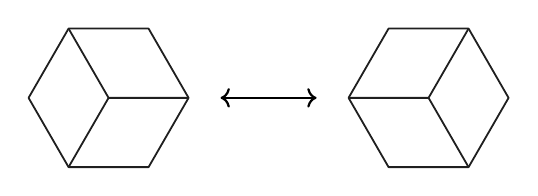
\begin{tikzpicture}[x=.40in,y=.40in]\HexBlues\begin{scope}[shift={(4,0)},rotate=60]\HexBlues\end{scope}\draw[<->,thick] (1.4,0)--(2.6,0);\end{tikzpicture}}
\newcommand{\StatePic}[2]{\begin{tikzpicture}[x=#2\blockside,y=#2\blockside]\csname Tiling#1\endcsname\draw[outline] \BoardPath;\draw[line width=2pt] (0,0)--(1,0);\end{tikzpicture}}
\newcommand{\StateCard}[1]{\begin{minipage}[t]{.30\linewidth}\centering\textbf{#1}\par\StatePic{#1}{.32}\end{minipage}}
% Generated by generate-geometry.py; coordinate unit = one small block edge.
\newcommand{\BoardGrid}{\draw[gridline] (-0.500000000,0.866025404)--(0.000000000,1.732050808)--(-1.000000000,1.732050808)--cycle;\draw[gridline] (-1.000000000,1.732050808)--(0.000000000,1.732050808)--(-0.500000000,2.598076211)--cycle;\draw[gridline] (0.000000000,1.732050808)--(0.500000000,2.598076211)--(-0.500000000,2.598076211)--cycle;\draw[gridline] (-0.500000000,2.598076211)--(0.500000000,2.598076211)--(0.000000000,3.464101615)--cycle;\draw[gridline] (0.500000000,2.598076211)--(1.000000000,3.464101615)--(0.000000000,3.464101615)--cycle;\draw[gridline] (0.000000000,0.000000000)--(0.500000000,0.866025404)--(-0.500000000,0.866025404)--cycle;\draw[gridline] (-0.500000000,0.866025404)--(0.500000000,0.866025404)--(0.000000000,1.732050808)--cycle;\draw[gridline] (0.500000000,0.866025404)--(1.000000000,1.732050808)--(0.000000000,1.732050808)--cycle;\draw[gridline] (0.000000000,1.732050808)--(1.000000000,1.732050808)--(0.500000000,2.598076211)--cycle;\draw[gridline] (1.000000000,1.732050808)--(1.500000000,2.598076211)--(0.500000000,2.598076211)--cycle;\draw[gridline] (0.500000000,2.598076211)--(1.500000000,2.598076211)--(1.000000000,3.464101615)--cycle;\draw[gridline] (0.000000000,0.000000000)--(1.000000000,0.000000000)--(0.500000000,0.866025404)--cycle;\draw[gridline] (1.000000000,0.000000000)--(1.500000000,0.866025404)--(0.500000000,0.866025404)--cycle;\draw[gridline] (0.500000000,0.866025404)--(1.500000000,0.866025404)--(1.000000000,1.732050808)--cycle;\draw[gridline] (1.500000000,0.866025404)--(2.000000000,1.732050808)--(1.000000000,1.732050808)--cycle;\draw[gridline] (1.000000000,1.732050808)--(2.000000000,1.732050808)--(1.500000000,2.598076211)--cycle;}
\newcommand{\TilingA}{\draw[tile] (-0.500000000,0.866025404)--(0.000000000,1.732050808)--(-0.500000000,2.598076211)--(-1.000000000,1.732050808)--cycle;\draw[tile] (0.000000000,1.732050808)--(0.500000000,2.598076211)--(0.000000000,3.464101615)--(-0.500000000,2.598076211)--cycle;\draw[tile] (0.500000000,2.598076211)--(1.500000000,2.598076211)--(1.000000000,3.464101615)--(0.000000000,3.464101615)--cycle;\draw[tile] (0.000000000,0.000000000)--(0.500000000,0.866025404)--(0.000000000,1.732050808)--(-0.500000000,0.866025404)--cycle;\draw[tile] (0.500000000,0.866025404)--(1.000000000,1.732050808)--(0.500000000,2.598076211)--(0.000000000,1.732050808)--cycle;\draw[tile] (1.000000000,1.732050808)--(2.000000000,1.732050808)--(1.500000000,2.598076211)--(0.500000000,2.598076211)--cycle;\draw[tile] (0.000000000,0.000000000)--(1.000000000,0.000000000)--(1.500000000,0.866025404)--(0.500000000,0.866025404)--cycle;\draw[tile] (0.500000000,0.866025404)--(1.500000000,0.866025404)--(2.000000000,1.732050808)--(1.000000000,1.732050808)--cycle;}
\newcommand{\PathA}{\draw[-{Stealth[length=4pt]},line width=1.2pt,dashed] (0.500000000,0.000000000)--(1.000000000,0.866025404);\draw[-{Stealth[length=4pt]},line width=1.2pt,dashed] (1.000000000,0.866025404)--(1.500000000,1.732050808);\draw[-{Stealth[length=4pt]},line width=1.2pt,dashed] (1.500000000,1.732050808)--(1.000000000,2.598076211);\draw[-{Stealth[length=4pt]},line width=1.2pt,dashed] (1.000000000,2.598076211)--(0.500000000,3.464101615);}
\newcommand{\TilingB}{\draw[tile] (-0.500000000,0.866025404)--(0.000000000,1.732050808)--(-0.500000000,2.598076211)--(-1.000000000,1.732050808)--cycle;\draw[tile] (0.000000000,1.732050808)--(0.500000000,2.598076211)--(0.000000000,3.464101615)--(-0.500000000,2.598076211)--cycle;\draw[tile] (0.500000000,2.598076211)--(1.500000000,2.598076211)--(1.000000000,3.464101615)--(0.000000000,3.464101615)--cycle;\draw[tile] (0.000000000,0.000000000)--(0.500000000,0.866025404)--(0.000000000,1.732050808)--(-0.500000000,0.866025404)--cycle;\draw[tile] (0.500000000,0.866025404)--(1.500000000,0.866025404)--(1.000000000,1.732050808)--(0.000000000,1.732050808)--cycle;\draw[tile] (0.000000000,1.732050808)--(1.000000000,1.732050808)--(1.500000000,2.598076211)--(0.500000000,2.598076211)--cycle;\draw[tile] (0.000000000,0.000000000)--(1.000000000,0.000000000)--(1.500000000,0.866025404)--(0.500000000,0.866025404)--cycle;\draw[tile] (1.500000000,0.866025404)--(2.000000000,1.732050808)--(1.500000000,2.598076211)--(1.000000000,1.732050808)--cycle;}
\newcommand{\PathB}{\draw[-{Stealth[length=4pt]},line width=1.2pt,dashed] (0.500000000,0.000000000)--(1.000000000,0.866025404);\draw[-{Stealth[length=4pt]},line width=1.2pt,dashed] (1.000000000,0.866025404)--(0.500000000,1.732050808);\draw[-{Stealth[length=4pt]},line width=1.2pt,dashed] (0.500000000,1.732050808)--(1.000000000,2.598076211);\draw[-{Stealth[length=4pt]},line width=1.2pt,dashed] (1.000000000,2.598076211)--(0.500000000,3.464101615);}
\newcommand{\TilingC}{\draw[tile] (-0.500000000,0.866025404)--(0.000000000,1.732050808)--(-0.500000000,2.598076211)--(-1.000000000,1.732050808)--cycle;\draw[tile] (0.000000000,1.732050808)--(0.500000000,2.598076211)--(0.000000000,3.464101615)--(-0.500000000,2.598076211)--cycle;\draw[tile] (0.500000000,2.598076211)--(1.500000000,2.598076211)--(1.000000000,3.464101615)--(0.000000000,3.464101615)--cycle;\draw[tile] (0.000000000,0.000000000)--(1.000000000,0.000000000)--(0.500000000,0.866025404)--(-0.500000000,0.866025404)--cycle;\draw[tile] (-0.500000000,0.866025404)--(0.500000000,0.866025404)--(1.000000000,1.732050808)--(0.000000000,1.732050808)--cycle;\draw[tile] (0.000000000,1.732050808)--(1.000000000,1.732050808)--(1.500000000,2.598076211)--(0.500000000,2.598076211)--cycle;\draw[tile] (1.000000000,0.000000000)--(1.500000000,0.866025404)--(1.000000000,1.732050808)--(0.500000000,0.866025404)--cycle;\draw[tile] (1.500000000,0.866025404)--(2.000000000,1.732050808)--(1.500000000,2.598076211)--(1.000000000,1.732050808)--cycle;}
\newcommand{\PathC}{\draw[-{Stealth[length=4pt]},line width=1.2pt,dashed] (0.500000000,0.000000000)--(0.000000000,0.866025404);\draw[-{Stealth[length=4pt]},line width=1.2pt,dashed] (0.000000000,0.866025404)--(0.500000000,1.732050808);\draw[-{Stealth[length=4pt]},line width=1.2pt,dashed] (0.500000000,1.732050808)--(1.000000000,2.598076211);\draw[-{Stealth[length=4pt]},line width=1.2pt,dashed] (1.000000000,2.598076211)--(0.500000000,3.464101615);}
\newcommand{\TilingD}{\draw[tile] (-0.500000000,0.866025404)--(0.000000000,1.732050808)--(-0.500000000,2.598076211)--(-1.000000000,1.732050808)--cycle;\draw[tile] (0.000000000,1.732050808)--(1.000000000,1.732050808)--(0.500000000,2.598076211)--(-0.500000000,2.598076211)--cycle;\draw[tile] (-0.500000000,2.598076211)--(0.500000000,2.598076211)--(1.000000000,3.464101615)--(0.000000000,3.464101615)--cycle;\draw[tile] (0.000000000,0.000000000)--(0.500000000,0.866025404)--(0.000000000,1.732050808)--(-0.500000000,0.866025404)--cycle;\draw[tile] (0.500000000,0.866025404)--(1.500000000,0.866025404)--(1.000000000,1.732050808)--(0.000000000,1.732050808)--cycle;\draw[tile] (1.000000000,1.732050808)--(1.500000000,2.598076211)--(1.000000000,3.464101615)--(0.500000000,2.598076211)--cycle;\draw[tile] (0.000000000,0.000000000)--(1.000000000,0.000000000)--(1.500000000,0.866025404)--(0.500000000,0.866025404)--cycle;\draw[tile] (1.500000000,0.866025404)--(2.000000000,1.732050808)--(1.500000000,2.598076211)--(1.000000000,1.732050808)--cycle;}
\newcommand{\PathD}{\draw[-{Stealth[length=4pt]},line width=1.2pt,dashed] (0.500000000,0.000000000)--(1.000000000,0.866025404);\draw[-{Stealth[length=4pt]},line width=1.2pt,dashed] (1.000000000,0.866025404)--(0.500000000,1.732050808);\draw[-{Stealth[length=4pt]},line width=1.2pt,dashed] (0.500000000,1.732050808)--(0.000000000,2.598076211);\draw[-{Stealth[length=4pt]},line width=1.2pt,dashed] (0.000000000,2.598076211)--(0.500000000,3.464101615);}
\newcommand{\TilingE}{\draw[tile] (-0.500000000,0.866025404)--(0.000000000,1.732050808)--(-0.500000000,2.598076211)--(-1.000000000,1.732050808)--cycle;\draw[tile] (0.000000000,1.732050808)--(1.000000000,1.732050808)--(0.500000000,2.598076211)--(-0.500000000,2.598076211)--cycle;\draw[tile] (-0.500000000,2.598076211)--(0.500000000,2.598076211)--(1.000000000,3.464101615)--(0.000000000,3.464101615)--cycle;\draw[tile] (0.000000000,0.000000000)--(1.000000000,0.000000000)--(0.500000000,0.866025404)--(-0.500000000,0.866025404)--cycle;\draw[tile] (-0.500000000,0.866025404)--(0.500000000,0.866025404)--(1.000000000,1.732050808)--(0.000000000,1.732050808)--cycle;\draw[tile] (1.000000000,1.732050808)--(1.500000000,2.598076211)--(1.000000000,3.464101615)--(0.500000000,2.598076211)--cycle;\draw[tile] (1.000000000,0.000000000)--(1.500000000,0.866025404)--(1.000000000,1.732050808)--(0.500000000,0.866025404)--cycle;\draw[tile] (1.500000000,0.866025404)--(2.000000000,1.732050808)--(1.500000000,2.598076211)--(1.000000000,1.732050808)--cycle;}
\newcommand{\PathE}{\draw[-{Stealth[length=4pt]},line width=1.2pt,dashed] (0.500000000,0.000000000)--(0.000000000,0.866025404);\draw[-{Stealth[length=4pt]},line width=1.2pt,dashed] (0.000000000,0.866025404)--(0.500000000,1.732050808);\draw[-{Stealth[length=4pt]},line width=1.2pt,dashed] (0.500000000,1.732050808)--(0.000000000,2.598076211);\draw[-{Stealth[length=4pt]},line width=1.2pt,dashed] (0.000000000,2.598076211)--(0.500000000,3.464101615);}
\newcommand{\TilingF}{\draw[tile] (-0.500000000,0.866025404)--(0.500000000,0.866025404)--(0.000000000,1.732050808)--(-1.000000000,1.732050808)--cycle;\draw[tile] (-1.000000000,1.732050808)--(0.000000000,1.732050808)--(0.500000000,2.598076211)--(-0.500000000,2.598076211)--cycle;\draw[tile] (-0.500000000,2.598076211)--(0.500000000,2.598076211)--(1.000000000,3.464101615)--(0.000000000,3.464101615)--cycle;\draw[tile] (0.000000000,0.000000000)--(1.000000000,0.000000000)--(0.500000000,0.866025404)--(-0.500000000,0.866025404)--cycle;\draw[tile] (0.500000000,0.866025404)--(1.000000000,1.732050808)--(0.500000000,2.598076211)--(0.000000000,1.732050808)--cycle;\draw[tile] (1.000000000,1.732050808)--(1.500000000,2.598076211)--(1.000000000,3.464101615)--(0.500000000,2.598076211)--cycle;\draw[tile] (1.000000000,0.000000000)--(1.500000000,0.866025404)--(1.000000000,1.732050808)--(0.500000000,0.866025404)--cycle;\draw[tile] (1.500000000,0.866025404)--(2.000000000,1.732050808)--(1.500000000,2.598076211)--(1.000000000,1.732050808)--cycle;}
\newcommand{\PathF}{\draw[-{Stealth[length=4pt]},line width=1.2pt,dashed] (0.500000000,0.000000000)--(0.000000000,0.866025404);\draw[-{Stealth[length=4pt]},line width=1.2pt,dashed] (0.000000000,0.866025404)--(-0.500000000,1.732050808);\draw[-{Stealth[length=4pt]},line width=1.2pt,dashed] (-0.500000000,1.732050808)--(0.000000000,2.598076211);\draw[-{Stealth[length=4pt]},line width=1.2pt,dashed] (0.000000000,2.598076211)--(0.500000000,3.464101615);}
\newcommand{\TriangleSolution}{\draw[tile,fill=white] (0.000000000,0.000000000)--(1.000000000,0.000000000)--(1.500000000,0.866025404)--(0.500000000,0.866025404)--cycle;\node[font=\small] at (0.750000000,0.433012702) {B};\draw[tile,fill=white] (1.000000000,0.000000000)--(2.000000000,0.000000000)--(2.500000000,0.866025404)--(1.500000000,0.866025404)--cycle;\node[font=\small] at (1.750000000,0.433012702) {B};\draw[tile,fill=white] (0.500000000,0.866025404)--(1.500000000,0.866025404)--(2.000000000,1.732050808)--(1.000000000,1.732050808)--cycle;\node[font=\small] at (1.250000000,1.299038106) {B};\draw[tile,fill=black!12] (2.000000000,0.000000000)--(3.000000000,0.000000000)--(2.500000000,0.866025404)--cycle;\node[font=\small] at (2.500000000,0.288675135) {G};\draw[tile,fill=black!12] (1.500000000,0.866025404)--(2.500000000,0.866025404)--(2.000000000,1.732050808)--cycle;\node[font=\small] at (2.000000000,1.154700538) {G};\draw[tile,fill=black!12] (1.000000000,1.732050808)--(2.000000000,1.732050808)--(1.500000000,2.598076211)--cycle;\node[font=\small] at (1.500000000,2.020725942) {G};}
\newcommand{\TrianglePurpleSolution}{\draw[tile,fill=white] (1.000000000,0.000000000)--(2.000000000,0.000000000)--(2.500000000,0.866025404)--(2.000000000,1.732050808)--(1.000000000,1.732050808)--(1.500000000,0.866025404)--cycle;\node[font=\small] at (1.950000000,0.866025404) {P};\draw[tile,fill=white] (0.000000000,0.000000000)--(1.000000000,0.000000000)--(1.500000000,0.866025404)--(0.500000000,0.866025404)--cycle;\node[font=\small] at (0.750000000,0.433012702) {B};\draw[tile,fill=black!12] (0.500000000,0.866025404)--(1.500000000,0.866025404)--(1.000000000,1.732050808)--cycle;\node[font=\small] at (1.000000000,1.154700538) {G};\draw[tile,fill=black!12] (1.000000000,1.732050808)--(2.000000000,1.732050808)--(1.500000000,2.598076211)--cycle;\node[font=\small] at (1.500000000,2.020725942) {G};\draw[tile,fill=black!12] (2.000000000,0.000000000)--(3.000000000,0.000000000)--(2.500000000,0.866025404)--cycle;\node[font=\small] at (2.500000000,0.288675135) {G};}
\newcommand{\Bottleneck}{\draw[tile] (0.000000000,0.000000000)--(1.000000000,0.000000000)--(0.500000000,0.866025404)--cycle;\node[font=\bfseries\small] at (0.500000000,0.288675135) {A};\draw[tile] (1.000000000,0.000000000)--(2.000000000,0.000000000)--(1.500000000,0.866025404)--cycle;\node[font=\bfseries\small] at (1.500000000,0.288675135) {B};\draw[tile] (0.500000000,0.866025404)--(1.500000000,0.866025404)--(1.000000000,1.732050808)--cycle;\node[font=\bfseries\small] at (1.000000000,1.154700538) {C};\draw[tile] (1.500000000,0.866025404)--(1.000000000,0.000000000)--(0.500000000,0.866025404)--cycle;\node[font=\bfseries\small] at (1.000000000,0.577350269) {D};\draw[tile] (1.000000000,1.732050808)--(0.500000000,0.866025404)--(0.000000000,1.732050808)--cycle;\node[font=\bfseries\small] at (0.500000000,1.443375673) {E};\draw[tile] (2.000000000,1.732050808)--(1.500000000,0.866025404)--(1.000000000,1.732050808)--cycle;\node[font=\bfseries\small] at (1.500000000,1.443375673) {F};}


% Generated by generate-k1-geometry.py. One coordinate unit = one small edge.
\newcommand{\KSailboatPath}{(0.000000000,0.000000000)--(3.000000000,0.000000000)--(3.500000000,0.866025404)--(2.500000000,0.866025404)--(1.500000000,2.598076211)--(0.500000000,0.866025404)--(-0.500000000,0.866025404)--cycle}
\newcommand{\KSailboatGreenSolution}{\draw[tile,fill=black!6] (-0.500000000,0.866025404)--(0.000000000,0.000000000)--(0.500000000,0.866025404)--cycle;\draw[tile,fill=black!6] (2.500000000,0.866025404)--(2.000000000,0.000000000)--(3.000000000,0.000000000)--cycle;\draw[tile,fill=black!6] (0.500000000,0.866025404)--(0.000000000,0.000000000)--(1.000000000,0.000000000)--cycle;\draw[tile,fill=black!6] (1.500000000,2.598076211)--(1.000000000,1.732050808)--(2.000000000,1.732050808)--cycle;\draw[tile,fill=black!6] (1.000000000,1.732050808)--(0.500000000,0.866025404)--(1.500000000,0.866025404)--cycle;\draw[tile,fill=black!6] (0.500000000,0.866025404)--(1.000000000,0.000000000)--(1.500000000,0.866025404)--cycle;\draw[tile,fill=black!6] (1.500000000,0.866025404)--(2.000000000,0.000000000)--(2.500000000,0.866025404)--cycle;\draw[tile,fill=black!6] (2.500000000,0.866025404)--(3.000000000,0.000000000)--(3.500000000,0.866025404)--cycle;\draw[tile,fill=black!6] (2.000000000,1.732050808)--(1.500000000,0.866025404)--(2.500000000,0.866025404)--cycle;\draw[tile,fill=black!6] (1.000000000,1.732050808)--(1.500000000,0.866025404)--(2.000000000,1.732050808)--cycle;\draw[tile,fill=black!6] (1.500000000,0.866025404)--(1.000000000,0.000000000)--(2.000000000,0.000000000)--cycle;}
\newcommand{\KCatPath}{(-1.000000000,0.000000000)--(1.000000000,0.000000000)--(1.500000000,0.866025404)--(1.000000000,1.732050808)--(0.500000000,0.866025404)--(-0.500000000,0.866025404)--(-1.000000000,1.732050808)--(-1.500000000,0.866025404)--cycle}
\newcommand{\KCatGreenSolution}{\draw[tile,fill=black!6] (-0.500000000,0.866025404)--(0.000000000,0.000000000)--(0.500000000,0.866025404)--cycle;\draw[tile,fill=black!6] (0.500000000,0.866025404)--(0.000000000,0.000000000)--(1.000000000,0.000000000)--cycle;\draw[tile,fill=black!6] (-1.000000000,1.732050808)--(-1.500000000,0.866025404)--(-0.500000000,0.866025404)--cycle;\draw[tile,fill=black!6] (-1.500000000,0.866025404)--(-1.000000000,0.000000000)--(-0.500000000,0.866025404)--cycle;\draw[tile,fill=black!6] (1.000000000,1.732050808)--(0.500000000,0.866025404)--(1.500000000,0.866025404)--cycle;\draw[tile,fill=black!6] (-0.500000000,0.866025404)--(-1.000000000,0.000000000)--(0.000000000,0.000000000)--cycle;\draw[tile,fill=black!6] (0.500000000,0.866025404)--(1.000000000,0.000000000)--(1.500000000,0.866025404)--cycle;}
\newcommand{\KHexagonPath}{(1.000000000,0.000000000)--(0.500000000,0.866025404)--(-0.500000000,0.866025404)--(-1.000000000,0.000000000)--(-0.500000000,-0.866025404)--(0.500000000,-0.866025404)--cycle}
\newcommand{\KHexagonGreenSolution}{\draw[tile,fill=black!6] (-0.500000000,0.866025404)--(0.000000000,0.000000000)--(0.500000000,0.866025404)--cycle;\draw[tile,fill=black!6] (0.500000000,0.866025404)--(0.000000000,0.000000000)--(1.000000000,0.000000000)--cycle;\draw[tile,fill=black!6] (-1.000000000,0.000000000)--(-0.500000000,-0.866025404)--(0.000000000,0.000000000)--cycle;\draw[tile,fill=black!6] (0.000000000,0.000000000)--(-0.500000000,-0.866025404)--(0.500000000,-0.866025404)--cycle;\draw[tile,fill=black!6] (-0.500000000,0.866025404)--(-1.000000000,0.000000000)--(0.000000000,0.000000000)--cycle;\draw[tile,fill=black!6] (0.000000000,0.000000000)--(0.500000000,-0.866025404)--(1.000000000,0.000000000)--cycle;}
\newcommand{\KHexagonBlueSolution}{\draw[tile,fill=black!6] (0.500000000,0.866025404)--(-0.500000000,0.866025404)--(-1.000000000,0.000000000)--(0.000000000,0.000000000)--cycle;\draw[tile,fill=black!6] (-1.000000000,0.000000000)--(-0.500000000,-0.866025404)--(0.500000000,-0.866025404)--(0.000000000,0.000000000)--cycle;\draw[tile,fill=black!6] (0.500000000,0.866025404)--(0.000000000,0.000000000)--(0.500000000,-0.866025404)--(1.000000000,0.000000000)--cycle;}
\newcommand{\KDiamondPath}{(0.000000000,0.000000000)--(2.000000000,0.000000000)--(3.000000000,1.732050808)--(1.000000000,1.732050808)--cycle}
\newcommand{\KDiamondGreenSolution}{\draw[tile,fill=black!6] (2.000000000,1.732050808)--(2.500000000,0.866025404)--(3.000000000,1.732050808)--cycle;\draw[tile,fill=black!6] (0.500000000,0.866025404)--(0.000000000,0.000000000)--(1.000000000,0.000000000)--cycle;\draw[tile,fill=black!6] (1.000000000,1.732050808)--(0.500000000,0.866025404)--(1.500000000,0.866025404)--cycle;\draw[tile,fill=black!6] (0.500000000,0.866025404)--(1.000000000,0.000000000)--(1.500000000,0.866025404)--cycle;\draw[tile,fill=black!6] (2.000000000,1.732050808)--(1.500000000,0.866025404)--(2.500000000,0.866025404)--cycle;\draw[tile,fill=black!6] (1.500000000,0.866025404)--(2.000000000,0.000000000)--(2.500000000,0.866025404)--cycle;\draw[tile,fill=black!6] (1.000000000,1.732050808)--(1.500000000,0.866025404)--(2.000000000,1.732050808)--cycle;\draw[tile,fill=black!6] (1.500000000,0.866025404)--(1.000000000,0.000000000)--(2.000000000,0.000000000)--cycle;}
\newcommand{\KDiamondBlueSolution}{\draw[tile,fill=black!6] (3.000000000,1.732050808)--(2.000000000,1.732050808)--(1.500000000,0.866025404)--(2.500000000,0.866025404)--cycle;\draw[tile,fill=black!6] (1.500000000,0.866025404)--(0.500000000,0.866025404)--(0.000000000,0.000000000)--(1.000000000,0.000000000)--cycle;\draw[tile,fill=black!6] (2.000000000,1.732050808)--(1.000000000,1.732050808)--(0.500000000,0.866025404)--(1.500000000,0.866025404)--cycle;\draw[tile,fill=black!6] (2.500000000,0.866025404)--(1.500000000,0.866025404)--(1.000000000,0.000000000)--(2.000000000,0.000000000)--cycle;}
\newcommand{\KArrowPath}{(0.000000000,0.000000000)--(2.000000000,0.000000000)--(2.500000000,0.866025404)--(2.000000000,1.732050808)--(0.000000000,1.732050808)--(0.500000000,0.866025404)--cycle}
\newcommand{\KArrowGreenSolution}{\draw[tile,fill=black!6] (1.500000000,0.866025404)--(1.000000000,0.000000000)--(2.000000000,0.000000000)--cycle;\draw[tile,fill=black!6] (0.500000000,0.866025404)--(0.000000000,0.000000000)--(1.000000000,0.000000000)--cycle;\draw[tile,fill=black!6] (1.000000000,1.732050808)--(0.500000000,0.866025404)--(1.500000000,0.866025404)--cycle;\draw[tile,fill=black!6] (0.500000000,0.866025404)--(1.000000000,0.000000000)--(1.500000000,0.866025404)--cycle;\draw[tile,fill=black!6] (2.000000000,1.732050808)--(1.500000000,0.866025404)--(2.500000000,0.866025404)--cycle;\draw[tile,fill=black!6] (1.500000000,0.866025404)--(2.000000000,0.000000000)--(2.500000000,0.866025404)--cycle;\draw[tile,fill=black!6] (1.000000000,1.732050808)--(1.500000000,0.866025404)--(2.000000000,1.732050808)--cycle;\draw[tile,fill=black!6] (0.000000000,1.732050808)--(0.500000000,0.866025404)--(1.000000000,1.732050808)--cycle;}
\newcommand{\KArrowBlueSolution}{\draw[tile,fill=black!6] (1.500000000,0.866025404)--(0.500000000,0.866025404)--(0.000000000,0.000000000)--(1.000000000,0.000000000)--cycle;\draw[tile,fill=black!6] (0.000000000,1.732050808)--(0.500000000,0.866025404)--(1.500000000,0.866025404)--(1.000000000,1.732050808)--cycle;\draw[tile,fill=black!6] (1.000000000,1.732050808)--(1.500000000,0.866025404)--(2.500000000,0.866025404)--(2.000000000,1.732050808)--cycle;\draw[tile,fill=black!6] (2.500000000,0.866025404)--(1.500000000,0.866025404)--(1.000000000,0.000000000)--(2.000000000,0.000000000)--cycle;}
\newcommand{\KArrowPurpleSolution}{\draw[tile,fill=black!6] (0.000000000,0.000000000)--(1.000000000,0.000000000)--(1.500000000,0.866025404)--(1.000000000,1.732050808)--(0.000000000,1.732050808)--(0.500000000,0.866025404)--cycle;\draw[tile,fill=black!6] (1.000000000,0.000000000)--(2.000000000,0.000000000)--(2.500000000,0.866025404)--(2.000000000,1.732050808)--(1.000000000,1.732050808)--(1.500000000,0.866025404)--cycle;}
\newcommand{\KStarPath}{(1.000000000,0.000000000)--(1.500000000,0.866025404)--(0.500000000,0.866025404)--(0.000000000,1.732050808)--(-0.500000000,0.866025404)--(-1.500000000,0.866025404)--(-1.000000000,0.000000000)--(-1.500000000,-0.866025404)--(-0.500000000,-0.866025404)--(0.000000000,-1.732050808)--(0.500000000,-0.866025404)--(1.500000000,-0.866025404)--cycle}
\newcommand{\KStarGreenSolution}{\draw[tile,fill=black!6] (-0.500000000,0.866025404)--(0.000000000,0.000000000)--(0.500000000,0.866025404)--cycle;\draw[tile,fill=black!6] (0.500000000,0.866025404)--(0.000000000,0.000000000)--(1.000000000,0.000000000)--cycle;\draw[tile,fill=black!6] (-0.500000000,-0.866025404)--(0.000000000,-1.732050808)--(0.500000000,-0.866025404)--cycle;\draw[tile,fill=black!6] (-1.000000000,0.000000000)--(-1.500000000,-0.866025404)--(-0.500000000,-0.866025404)--cycle;\draw[tile,fill=black!6] (0.000000000,1.732050808)--(-0.500000000,0.866025404)--(0.500000000,0.866025404)--cycle;\draw[tile,fill=black!6] (0.000000000,0.000000000)--(0.500000000,-0.866025404)--(1.000000000,0.000000000)--cycle;\draw[tile,fill=black!6] (0.500000000,0.866025404)--(1.000000000,0.000000000)--(1.500000000,0.866025404)--cycle;\draw[tile,fill=black!6] (1.000000000,0.000000000)--(0.500000000,-0.866025404)--(1.500000000,-0.866025404)--cycle;\draw[tile,fill=black!6] (-1.000000000,0.000000000)--(-0.500000000,-0.866025404)--(0.000000000,0.000000000)--cycle;\draw[tile,fill=black!6] (0.000000000,0.000000000)--(-0.500000000,-0.866025404)--(0.500000000,-0.866025404)--cycle;\draw[tile,fill=black!6] (-0.500000000,0.866025404)--(-1.000000000,0.000000000)--(0.000000000,0.000000000)--cycle;\draw[tile,fill=black!6] (-1.500000000,0.866025404)--(-1.000000000,0.000000000)--(-0.500000000,0.866025404)--cycle;}
\newcommand{\KStarBlueSolution}{\draw[tile,fill=black!6] (0.000000000,1.732050808)--(-0.500000000,0.866025404)--(0.000000000,0.000000000)--(0.500000000,0.866025404)--cycle;\draw[tile,fill=black!6] (0.000000000,0.000000000)--(-1.000000000,0.000000000)--(-1.500000000,-0.866025404)--(-0.500000000,-0.866025404)--cycle;\draw[tile,fill=black!6] (0.000000000,0.000000000)--(-0.500000000,-0.866025404)--(0.000000000,-1.732050808)--(0.500000000,-0.866025404)--cycle;\draw[tile,fill=black!6] (1.500000000,0.866025404)--(0.500000000,0.866025404)--(0.000000000,0.000000000)--(1.000000000,0.000000000)--cycle;\draw[tile,fill=black!6] (0.000000000,0.000000000)--(0.500000000,-0.866025404)--(1.500000000,-0.866025404)--(1.000000000,0.000000000)--cycle;\draw[tile,fill=black!6] (-1.500000000,0.866025404)--(-1.000000000,0.000000000)--(0.000000000,0.000000000)--(-0.500000000,0.866025404)--cycle;}
\newcommand{\KStarPurpleSolution}{\draw[tile,fill=black!6] (0.000000000,1.732050808)--(-0.500000000,0.866025404)--(0.000000000,0.000000000)--(1.000000000,0.000000000)--(1.500000000,0.866025404)--(0.500000000,0.866025404)--cycle;\draw[tile,fill=black!6] (1.500000000,-0.866025404)--(1.000000000,0.000000000)--(0.000000000,0.000000000)--(-0.500000000,-0.866025404)--(0.000000000,-1.732050808)--(0.500000000,-0.866025404)--cycle;\draw[tile,fill=black!6] (-1.500000000,-0.866025404)--(-0.500000000,-0.866025404)--(0.000000000,0.000000000)--(-0.500000000,0.866025404)--(-1.500000000,0.866025404)--(-1.000000000,0.000000000)--cycle;}
\newcommand{\KLongHexagonPath}{(0.000000000,0.000000000)--(2.000000000,0.000000000)--(2.500000000,0.866025404)--(2.000000000,1.732050808)--(0.000000000,1.732050808)--(-0.500000000,0.866025404)--cycle}
\newcommand{\KLongHexagonGreenSolution}{\draw[tile,fill=black!6] (-0.500000000,0.866025404)--(0.000000000,0.000000000)--(0.500000000,0.866025404)--cycle;\draw[tile,fill=black!6] (1.500000000,0.866025404)--(1.000000000,0.000000000)--(2.000000000,0.000000000)--cycle;\draw[tile,fill=black!6] (0.500000000,0.866025404)--(0.000000000,0.000000000)--(1.000000000,0.000000000)--cycle;\draw[tile,fill=black!6] (1.000000000,1.732050808)--(0.500000000,0.866025404)--(1.500000000,0.866025404)--cycle;\draw[tile,fill=black!6] (0.500000000,0.866025404)--(1.000000000,0.000000000)--(1.500000000,0.866025404)--cycle;\draw[tile,fill=black!6] (1.500000000,0.866025404)--(2.000000000,0.000000000)--(2.500000000,0.866025404)--cycle;\draw[tile,fill=black!6] (0.000000000,1.732050808)--(-0.500000000,0.866025404)--(0.500000000,0.866025404)--cycle;\draw[tile,fill=black!6] (2.000000000,1.732050808)--(1.500000000,0.866025404)--(2.500000000,0.866025404)--cycle;\draw[tile,fill=black!6] (1.000000000,1.732050808)--(1.500000000,0.866025404)--(2.000000000,1.732050808)--cycle;\draw[tile,fill=black!6] (0.000000000,1.732050808)--(0.500000000,0.866025404)--(1.000000000,1.732050808)--cycle;}
\newcommand{\KLongHexagonBlueSolution}{\draw[tile,fill=black!6] (0.000000000,1.732050808)--(-0.500000000,0.866025404)--(0.000000000,0.000000000)--(0.500000000,0.866025404)--cycle;\draw[tile,fill=black!6] (1.500000000,0.866025404)--(0.500000000,0.866025404)--(0.000000000,0.000000000)--(1.000000000,0.000000000)--cycle;\draw[tile,fill=black!6] (2.500000000,0.866025404)--(1.500000000,0.866025404)--(1.000000000,0.000000000)--(2.000000000,0.000000000)--cycle;\draw[tile,fill=black!6] (1.000000000,1.732050808)--(1.500000000,0.866025404)--(2.500000000,0.866025404)--(2.000000000,1.732050808)--cycle;\draw[tile,fill=black!6] (0.000000000,1.732050808)--(0.500000000,0.866025404)--(1.500000000,0.866025404)--(1.000000000,1.732050808)--cycle;}
\newcommand{\KMountainPath}{(0.000000000,0.000000000)--(3.000000000,0.000000000)--(1.500000000,2.598076211)--cycle}
\newcommand{\KMountainGreenSolution}{\draw[tile,fill=black!6] (2.500000000,0.866025404)--(2.000000000,0.000000000)--(3.000000000,0.000000000)--cycle;\draw[tile,fill=black!6] (0.500000000,0.866025404)--(0.000000000,0.000000000)--(1.000000000,0.000000000)--cycle;\draw[tile,fill=black!6] (1.500000000,2.598076211)--(1.000000000,1.732050808)--(2.000000000,1.732050808)--cycle;\draw[tile,fill=black!6] (1.000000000,1.732050808)--(0.500000000,0.866025404)--(1.500000000,0.866025404)--cycle;\draw[tile,fill=black!6] (0.500000000,0.866025404)--(1.000000000,0.000000000)--(1.500000000,0.866025404)--cycle;\draw[tile,fill=black!6] (2.000000000,1.732050808)--(1.500000000,0.866025404)--(2.500000000,0.866025404)--cycle;\draw[tile,fill=black!6] (1.500000000,0.866025404)--(2.000000000,0.000000000)--(2.500000000,0.866025404)--cycle;\draw[tile,fill=black!6] (1.000000000,1.732050808)--(1.500000000,0.866025404)--(2.000000000,1.732050808)--cycle;\draw[tile,fill=black!6] (1.500000000,0.866025404)--(1.000000000,0.000000000)--(2.000000000,0.000000000)--cycle;}

\hypersetup{pdftitle={Week 1: Tiling, invariants, and local moves - facilitator guide}}
\begin{document}
\PageTitle{FACILITATOR}{Small pieces, serious questions}
\RuleBox{\textbf{The mathematical questions:} Can a region be tiled? What prevents a tiling? What is the least uncovered space? Can small swaps connect all solutions, and how many swaps are necessary?}
\Subhead{Your kits and the print scale}
These activities use \textbf{21st Century Pattern Blocks and the 1\(\times\) pieces from Upscale sets}. Core tasks specify the permitted shapes. Put 2\(\times\) and 3\(\times\) pieces aside until the scaling extension. No square block is needed.

The default edge is \textbf{1 inch (25.4 mm)}. The designer describes the sets as compatible with traditional blocks and identifies one-inch short edges in his 21st Century mosaic. Your measured green edge is also approximately one inch. This supports the nominal scale; it does not resolve 25 versus 25.4 mm for an individual batch. Print \textbf{US Letter, single-sided, 100\% / Actual Size} and match the check line with a small green triangle.

If the fit is noticeably off, trace your physical \textbf{2\(\times\) and 3\(\times\) green triangles} for the middle-group boundaries. For the upper board, trace one of the displayed eight-rhombus constructions. Or set \texttt{\textbackslash blockside} in \texttt{common.tex} to the measured edge and rebuild. Do not let a printer-fit problem become a puzzle about gaps.
\Subhead{Prepare for the seven children}
Per K--1 child: 3 purple chevrons, 12 greens, 6 blues, and a few reds and yellows for mixed fillings. Reuse pieces from one outline to the next. Per middle child: 3 blues, 3 greens, 1 purple, and 2 pink right triangles. Upper child: 8 blues, pencil, and optionally string to trace a ribbon. Across the kits, gather \textbf{35 small blues, 45 greens, and 12 purples}. The optional paper-rhombus sheet supplies 12 extra blues if needed.

One standard 21st Century box has 18 blues, 24 greens, 12 purples, 24 pinks, 12 reds, 12 yellows, 18 teal kites, and 12 gray darts (manufacturer booklet, p. 2). Your additional Upscale sets can supply the extra small blues and greens. Check that edges match across batches.
\Subhead{Readiness and a flexible hour}
\textbf{K--1:} Match edges and rotate pieces; no independent reading, writing, or arithmetic. Explore how different pieces fill the same boundary.\par
\textbf{2--3:} Count and compare up to nine spaces; distinguish finding a packing from explaining why nobody can improve it. No fractions or formulas.\par
\textbf{4--5:} Track arrangements and legal moves; reason about an exhaustive list, shortest paths, and odd/even returns. No probability prerequisite.

\textbf{0--10:} Free construction, including the extra shapes. \textbf{10--15:} Launch: ``Can you fill this outline?'' Let children place the first pieces. \textbf{15--35:} Group investigations. \textbf{35--40:} Movement/reset. \textbf{40--55:} Continue or choose another mat. \textbf{55--60:} Share one reason, surprise, or question; tidy up.

Give one page at a time. Keep one adult mainly with K--1; the organizer starts the middle and upper work and returns for explanations. The fifth grader should get a real discussion about the best route. Let the upper child record discoveries on the nine blank boards (page 2) before giving the six reference cards (page 3). Do not require completion of every page.
\newpage
\PageTitle{FACILITATOR}{Fillings, obstructions, and repair}
\Subhead{K--1: fill, lift, and fill again / F01-K-v3}
\textbf{Page 1:} free filling; the sailboat takes 11 greens, the cat 7. \textbf{Page 2:} a hexagon takes 1 yellow, 3 blues, or 6 greens; a diamond takes 4 blues or 8 greens. Trace joins, lift, and reuse pieces. Different piece types count as another way. \textbf{Page 3:} arrow = 2 purples; star = 3. Show only a starting piece if needed.
\begin{center}\begin{minipage}[c]{1.3in}\centering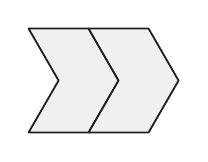
\begin{tikzpicture}[x=.30in,y=.30in]\KArrowPurpleSolution\end{tikzpicture}\end{minipage}\hspace{.25in}\begin{minipage}[c]{1.3in}\centering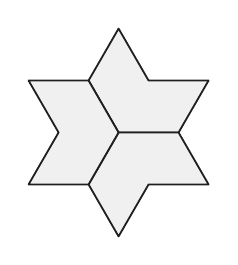
\begin{tikzpicture}[x=.30in,y=.30in]\KStarPurpleSolution\end{tikzpicture}\end{minipage}\end{center}
\textbf{Page 4:} long hexagon = 5 blues; mountain = 9 greens. Refill freely afterward. \textbf{Hints:} ``Which piece fits this corner?'' ``Try turning it.'' \textbf{Ask:} ``Can you fill it another way?'' A checked filling is a satisfying stop. No impossible mats, minimum-piece goals, or flip rules. Offer the existing 2--3 packet for harder work.
\Subhead{Middle page 1: area alone does not decide tileability}
Board B is two blues side by side. Board A is a side-two triangle: it has \textbf{3 up-pointing and 1 down-pointing spaces}. Every allowed blue covers \textbf{one of each}, in any orientation. Two blues would need two down spaces, but only one exists. Repeated attempts cannot change this count.

Let children try, talk together, and develop their own reasons. Keep hints in reserve. If needed, invite them to copy a blue with two greens: ``What kinds of spaces does a blue always cover, even when you turn it?'' They can shade up spaces or mark them with dots. A later discussion prompt: ``Can you explain why more tries will not change one board's answer?'' Equal up/down counts are \emph{necessary}, not sufficient; see the reserve on page 5.
\textbf{Satisfying stop:} Tile B and explain why A cannot tile. \textbf{Optional proof:} Match a three-gap construction on T3 with a bound showing fewer gaps are impossible.
\Subhead{Middle page 2: an optimum needs two arguments}
The side-three triangle has \textbf{6 up and 3 down spaces}. At most three blues fit, leaving at least three spaces. The construction below attains that bound: \textbf{3 blues + 3 greens}. Thus the fewest gaps, or the fewest small green fillers, is \textbf{3}.
\begin{center}
\begin{minipage}{.44\linewidth}\centering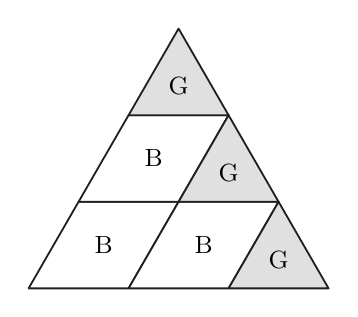
\begin{tikzpicture}[x=.50in,y=.50in]\TriangleSolution\end{tikzpicture}\par 3 blues + 3 greens\end{minipage}\hfill
\begin{minipage}{.44\linewidth}\centering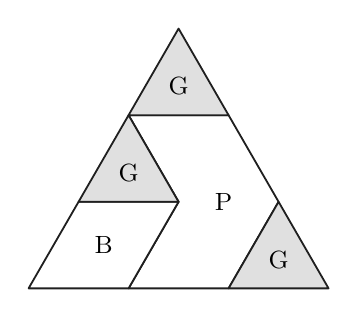
\begin{tikzpicture}[x=.50in,y=.50in]\TrianglePurpleSolution\end{tikzpicture}\par With purple (page 3): 5 blocks\end{minipage}
\end{center}
\textbf{Generalization:} Each horizontal row has one more up than down space. A side-\(n\) triangle therefore needs at least \(n\) greens. Pair each down space with the up space immediately below-left of it; the unpaired up spaces along the right edge give a construction using exactly \(n\) greens. In symbols, the up/down counts are \(n(n+1)/2\) and \(n(n-1)/2\); the row argument needs no formulas.
\newpage
\PageTitle{FACILITATOR}{When the pieces change}
\Subhead{Middle page 3: purple cannot improve the gap count}
Every purple can be replaced by two blues covering exactly the same region. If blues and purples left fewer than three gaps on the big triangle, replacing the purples would give an all-blue packing with the same gaps. But page 2 proved that impossible. This is a small \textbf{reduction}: a supposedly better packing would also solve the old impossible problem.

The same replacement shows that purples cannot tile Board A or lower the minimum of \(n\) small green fillers in a side-\(n\) triangle. On T3, however, the \emph{total block count} falls from six to \textbf{five}: one purple, one blue, three greens (see page 2). Four blocks cannot work: at least three must be greens, leaving at most one purple, for an area of at most seven, short of nine. Name exactly which quantity is being minimized.
\Subhead{Pink does rescue it: a theorem has assumptions}
Two pink right triangles fill Board A, meeting along its altitude:
\begin{center}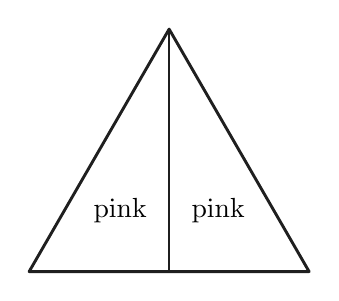
\begin{tikzpicture}[x=.70in,y=.70in]\draw[outline] (0,0)--(2,0)--(1,2*\hh)--cycle;\draw[tile] (1,0)--(1,2*\hh);\node at (.65,.5*\hh) {pink};\node at (1.35,.5*\hh) {pink};\end{tikzpicture}\end{center}
Each pink has side lengths \(1,\sqrt3,2\) small-edge units, so it is half a side-two equilateral triangle. It cuts across the unit-cell grid, rather than covering whole up/down spaces. The obstruction holds for blues and purples, but its premise fails for pink. Invite children to point to the split cell. The discussion takeaway: an impossibility argument must say \textbf{which pieces} are allowed.
\Subhead{Upper pages 1--3: the complete world has six states}
The board has sides \(1,2,2,1,2,2\), area 16 small triangles, and eight blues in every tiling. Keep the marked bottom edge fixed. The reference cards display all six possibilities, but the cards alone do not prove completeness. Until the ribbon argument on page 4, label completeness as \emph{supplied} or \emph{awaiting proof}. Check the cards' legal flips:
\begin{center}\begin{tikzpicture}[x=1in,y=.6in,every node/.style={circle,draw,minimum size=24pt,font=\bfseries}]
\node(A)at(0,0){A};\node(B)at(1,0){B};\node(C)at(2,1){C};\node(D)at(2,-1){D};\node(E)at(3,0){E};\node(F)at(4,0){F};
\draw (A)--(B)--(C)--(E)--(F) (B)--(D)--(E);
\end{tikzpicture}\end{center}
\textbf{Shortest A to F:} four flips, by A--B--C--E--F or A--B--D--E--F. A route must leave A through B, reach E before F, and get from B to E in at least two moves. The graph therefore supplies both a lower bound and matching routes.

\textbf{No odd return:} Separate the states into \{A,C,D,F\} and \{B,E\}. Every edge crosses between groups. An odd number of flips ends in the other group; an even number is necessary to return. ``I tried several odd routes'' alone is not a proof.
\textbf{Satisfying stop:} Explain a shortest route in the supplied six-state graph. \textbf{Optional proof:} Use ribbons to exclude a seventh tiling, or prove the odd-return obstruction. Record which claim the child actually explained.
\newpage
\PageTitle{FACILITATOR}{Why there is no seventh state}
\Subhead{A concrete code for every tiling}
Follow a ribbon from the midpoint of the bold bottom side: cross the rhombus to its opposite horizontal side, then cross the next rhombus upward, until reaching the top. The four crossings go either right (R) or left (L). The total rise and matching horizontal endpoints force \textbf{two R's and two L's}.
\begin{center}
\begin{minipage}{.30\linewidth}\centering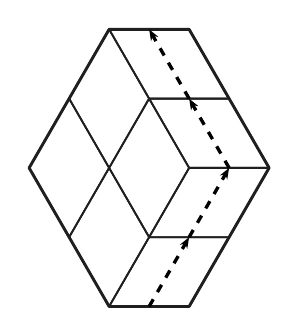
\begin{tikzpicture}[x=.40in,y=.40in]\TilingA\draw[outline] \BoardPath;\PathA\end{tikzpicture}\par A: RRLL\end{minipage}\hfill
\begin{minipage}{.30\linewidth}\centering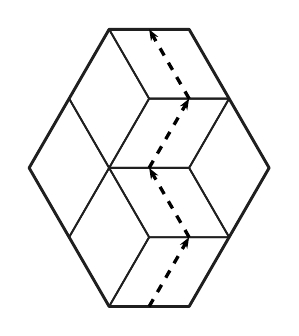
\begin{tikzpicture}[x=.40in,y=.40in]\TilingB\draw[outline] \BoardPath;\PathB\end{tikzpicture}\par B: RLRL\end{minipage}\hfill
\begin{minipage}{.30\linewidth}\centering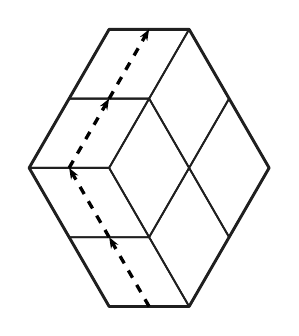
\begin{tikzpicture}[x=.40in,y=.40in]\TilingF\draw[outline] \BoardPath;\PathF\end{tikzpicture}\par F: LLRR\end{minipage}
\end{center}
There is only one such ribbon: following any rhombus with horizontal sides downward must reach the sole horizontal bottom side, and downward steps cannot cycle. Once the ribbon is fixed, every remaining rhombus has the third orientation. Each remaining triangle has at most one partner in that orientation, so those placements are forced.

The only possible orders, and the cards realizing them, are:
\begin{center}\begin{tabular}{c|cccccc}
Card&A&B&C&D&E&F\\\hline
Ribbon&RRLL&RLRL&LRRL&RLLR&LRLR&LLRR\\
Score&0&1&2&2&3&4
\end{tabular}\end{center}
List the possibilities by the positions of the two L's: 12, 13, 14, 23, 24, 34. All six orders occur, so there are exactly six tilings. There is no hidden disconnected seventh state. Use string or a finger on the pictures before introducing the letter code.
\Subhead{A second proof of the minimum number of flips}
A flip swaps neighboring unlike letters: RL becomes LR or the reverse. Give a ribbon one point for each pair where an L occurs earlier than an R. RRLL scores 0; LLRR scores 4. One swap changes only the relative order of those two letters, changing the score by exactly 1. At least four flips are needed, and the displayed routes attain four.

This is a small instance of a \textbf{height function}: a number tracks progress and bounds what a local move can accomplish. For a child, the score or the two graph groups may be enough. The full research height construction is an adult extension, not prerequisite notation.
\Subhead{Hints without doing the investigation for them}
If the middle group's purple discussion stalls, offer: ``Build a purple from blues. What does that tell you about the fewest gaps?''

If filling the board stalls, give just card A to copy. If flips are hard to see, outline a little yellow-hexagon-sized patch in the drawing. If the graph is incomplete, compare two cards and ask which pieces changed. If shortest-path reasoning stalls, ask which state must come just after A and just before F. If the ribbon is too abstract, stay with the actual six-card graph.
\newpage
\PageTitle{FACILITATOR}{Where these questions lead}
\Subhead{A balanced board can still fail / reserve}
\begin{minipage}[c]{.34\linewidth}\centering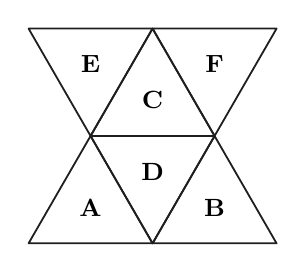
\begin{tikzpicture}[x=.62in,y=.62in]\Bottleneck\end{tikzpicture}\end{minipage}\hfill
\begin{minipage}[c]{.62\linewidth}This region has three up and three down cells. Yet A and B can each pair only with D; both cannot have it. It has no blue tiling. Two blues on A+D and C+E, with greens at B and F, attain the minimum of two green fillers. This is a concrete \textbf{Hall matching obstruction}.\end{minipage}
\Subhead{Use the Upscale pieces deliberately / reserve}
Scale the entire small-hexagon puzzle by 2 and use three 2\(\times\) blues: its two tilings are unchanged in structure. Keep the same 2\(\times\) yellow outline but switch to 1\(\times\) blues: twelve pieces are required, and there are \textbf{20} tilings. Refining the pieces creates new configurations; merely scaling everything does not. For a later visit, try to find tilings that do not group back into three large blues.
\Subhead{Two random-flip rules}
If each step chooses uniformly among \emph{currently legal} flips, the six states have degrees \(1,3,2,2,3,1\). Long-run visit frequencies are those numbers divided by 12. The mean first positive return to A is \textbf{12 moves}, not six. The walk has period two; that does not invalidate the return-time result.

A different rule chooses uniformly among the four possible interior flip centers; if the chosen center cannot flip, count a turn and stay. Transition probabilities are symmetric, so uniform occupancy and mean first positive return \textbf{6 turns} follow. A stay counts as an immediate return. This distinction is itself a worthwhile later investigation; it is not in the core K--5 hour.
\Subhead{Research and undergraduate lineage}
\textbf{Thurston, \emph{Conway's Tiling Groups} (1990), pp. 757--773, especially p. 767:} boundary information and height surfaces for tileability. \href{https://www.ibr.cs.tu-bs.de/users/fekete/oldhp/Sem06/thurston.pdf}{University-hosted original paper}.\par
\textbf{Saldanha--Tomei, \emph{An overview of domino and lozenge tilings}, \S3, Theorems 3.1--3.2:} connectivity and minimum flip distance for simply connected regions. \href{https://arxiv.org/pdf/math/9801111}{Author manuscript}. Holes and mixed tile sets require new arguments.\par
\textbf{MIT undergraduate discrete mathematics:} Postnikov's 18.312 lectures 20--23 cover tilings, matchings, Hall's theorem, and plane partitions. Levin's \emph{Discrete Mathematics: An Open Introduction}, \S2.7, treats matching obstructions. MIT \emph{Mathematics for Computer Science}, \S5.1.5, develops recursive L-tromino tiling of deficient power-of-two square boards; keep that as a separate paper-grid session.\par
\textbf{Further research:} Cohn--Larsen--Propp (1998) study typical boxed plane partitions; Wilson (2004) studies lozenge dynamics and card shuffling. The research notes in \texttt{plans/} give primary links, precise hypotheses, and checked finite constructions.

\textbf{Teaching and kit sources:} Math for Love's 21st Century booklet p. 2; Danielson's \emph{Five fun things} and \emph{Minnesota's Largest Pattern Block Mosaic}; JRMF \emph{Changing Colors}, pp. 3--6; \emph{Math Circle by the Bay}, preface pp. ix--x. K--1 mat-making also draws on EFM's \emph{Pattern Blocks -- Least Pieces}, p. 1 (without its optimization goal), and the prior Lowell \emph{Pattern Block Exercises}, p. 1. Our eight outlines are new constructions. Record actual use as F01-K-v3/M-v2/U-v2; do not mark reserve pages as taught.
\end{document}
